\section{Applying the platform to the OLAF problem}

The problem of creating an address file for the UK was described in \ref{subs:the-problem-of-creating-an-olaf}. This section describes a possible workflow that can be implemented on the platform and how some of its parts were implemented for evaluation.

\subsection{How the primary open data sources shape the problem}

The availability of reliable relevant open data is central to the definition of the workflow, as it is the main assumption of the work that the best possible use of computation and crowdsourcing is to complement published data rather than creating it from scratch [I THOUGHT I HAD WRITTEN THIS IN THE DOCUMENT BEFORE, WHERE IS IT?]. 

An assessment of what open data sources were available, made at the time this work was performed, made it possible to consider solving the OLAF problem equivalent to solving three sub-problems {\it p1}, {\it p2} and {\it p3} centred around the same dataset: Ordnance Survey's "Open Names"\footnote{Ordnance Survey is the national mapping agency for Great Britain. See \url{https://www.ordnancesurvey.co.uk/business-and-government/products/os-open-names.html} (referred to as "OSON" in the following), as described below:

\begin{figure}[!h]
    \begin{floatrow}
        \ffigbox{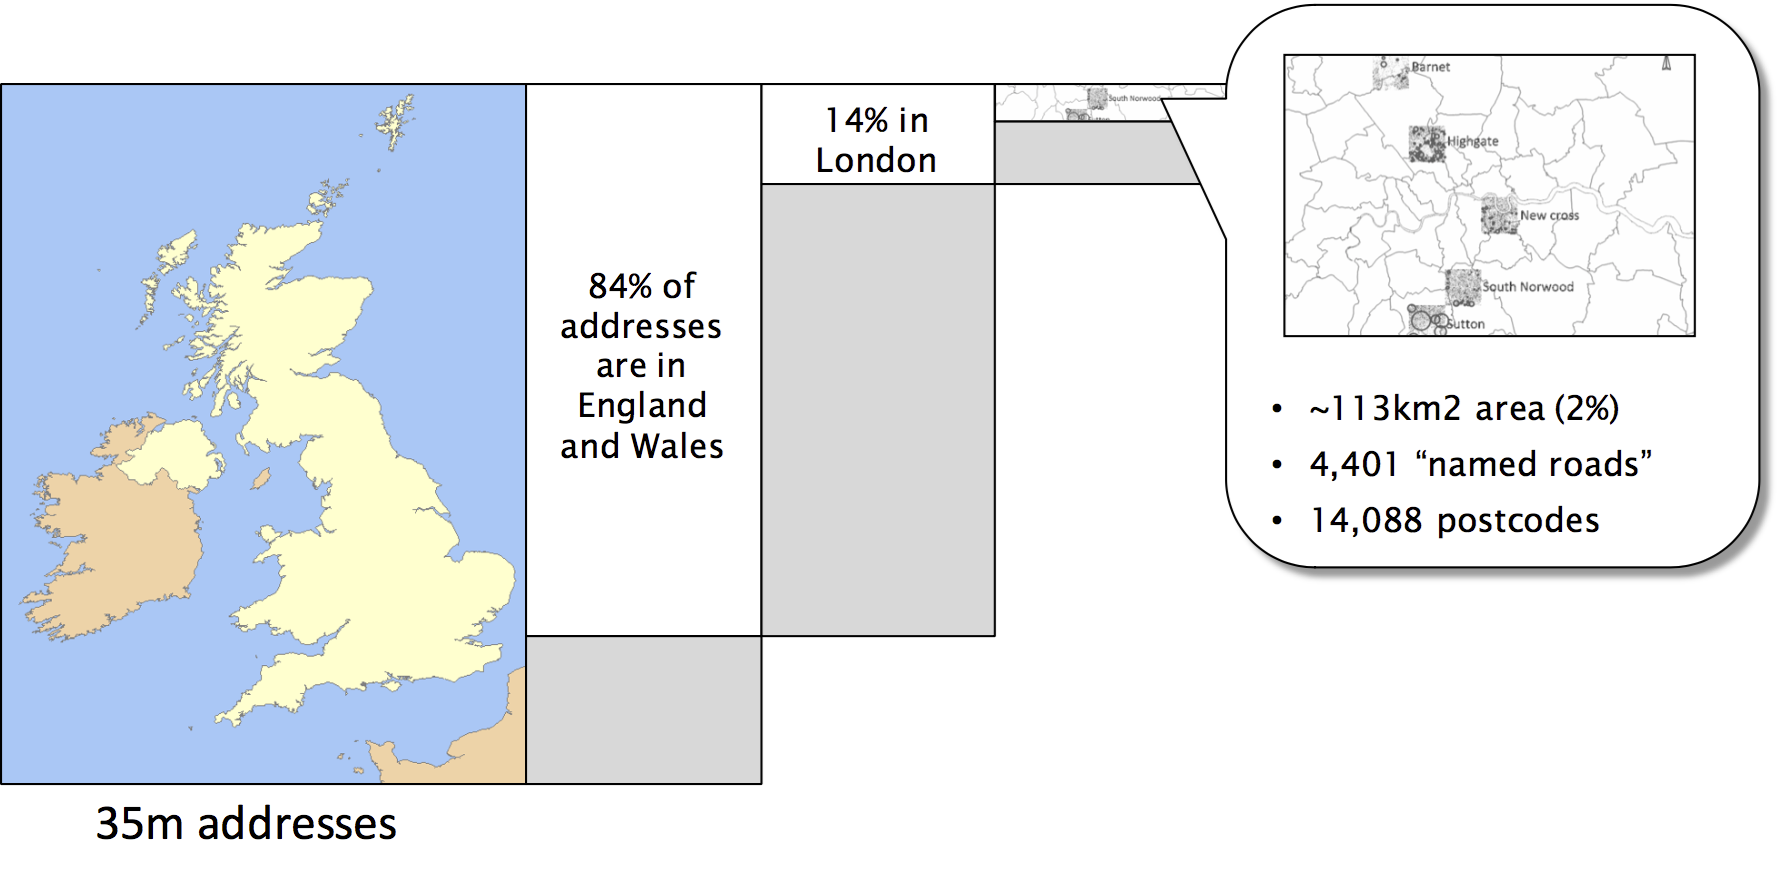
\includegraphics[width=1.0\textwidth]{social-machine-mix-3.png}}{\caption{Applicability of address inference - General statistics}\label{fig:social_machine_mix_3}}
   \end{floatrow}
\end{figure}
        
    
\begin{itemize}
    \item {\it p1}: Create a list of all existing {\it house numbers} for each road listed in OSON.
    \item {\it p2}: Create a list of all existing {\it house names} for each road listed in OSON.
    \item {\it p3}: Create a list of the associations between each of the house numbers and names above and the list of current\footnote{Postcodes can change. The problem of documenting how addresses change postcode in time is relevant but outside of the scope of research.} postcodes in OSON. 
\end{itemize}

For simplicity, in the following the terms "place", "road" and "street" are used interchangeably, as they are equivalent in OLAF from a data model perspective.

OSON "lists definitive place names, roads numbers and postcodes in Great Britain".} and is instrumental to the work as it is the open dataset that is closer to the target, contentwise. In other words, OLAF can be seen as an augmentation of OSON, obtained by adding just one dimension to what can be already found in it, that is the list of house names and numbers associated to each of its roads and postcodes. 
    
Problems {\it p2}\footnote{Note that 98\% of UK addresses are characterised by a house number rather than a house name, so solving {\it p1} is substantially more relevant to achieve completeness in OLAF than {\it p2}.} and {\it p3} are not discussed further in this paper. 

\subsection{Creating a list of all existing house numbers for each road listed in OSON} 

Problem {\it p1} can be further decomposed in four sub-problems, thanks to the availability of additional open data sources:
    
\begin{itemize}
    \item {\it p1.1}: Identify the list of house numbers in each OSON road through references in other open data.
    \item {\it p1.2}: Statistically infer the existence of house numbers from the house numbers collected at {\it p1.1}.
    \item {\it p1.3}: Enable the further application of {\it p1.2} by creating the necessary data through crowdsourcing.
    \item {\it p1.4}: Correct the output of {\it p1.3}.
\end{itemize}

\textbf{House numbers from references in other open data} References to existing house names and numbers can be found in several open data publications in the UK. The largest in size, and the one used in the experiments, is Land Registry's "Price Paid Data"\footnote{Land Registry is a non-ministerial UK Government department with the responsibility to register the ownership of land and property in England and Wales. See \url{https://www.gov.uk/government/collections/price-paid-data}.} ("LRPP" in the following). LRPP records every property ownership transfer in England and Wales since 1995, including its full address.

\textbf{House number inference} Each culture developed in time a convention for the assignment of house number and names to buildings. In the UK, it is reported that numbering was likely introduced in the early 18th Century as an alternative to house names. Buildings typically are numbered sequentially starting from 1, corresponding to the extremity of the road that is closest to the centre of the town the street belongs to. Odd numbers are on the left-hand side as seen from the centre, even number on the right-hand side. Intermediate properties usually have a number suffixed by one or more letters, this is typical of larger buildings that at some point in time got divided into more smaller dwellings. 
        
Algorithms \ref{algo:inference-numbers} and \ref{algo:inference-numbers-suffix} below apply this understanding of the numbering system and have a very high probability to infer correctly the existence of house numbers from other known house numbers\footnote{It should be remembered, though, that centuries of house development and using the described numbering system loosely of course created many exceptions: e.g. there are buildings in the UK whose house number is zero, places where numbers were assigned consecutively on the same side of the street, and house numbers that are simply missing etc. Other available open data sources enable more complex algorithms, e.g. Ordnance Survey's "Open Maps - Local" includes summary shapes for the buildings in each street, hence enabling the detection of how many buildings are present and hint at which house numbers may be missing.}. Although a few house numbers will be inferred in error, \footnote{Error is caused by three cases: (i) inferred house numbers for buildings that use house names (ii) inferred house numbers that in reality exist only in suffixed form (e.g. 7A instead of 7), and (iii) addresses that are simply missing, e.g. because a building was demolished. We can estimate (i) and (ii) by observing the occurrence of the cases in LRPP. For (i), the frequency of addresses identified by house names instead than house numbers is 2\% of the total for the sampled geographic area. For (ii), the probability that a house number is used only in suffixed format is 2.6\% and that it is used also in suffixed format an additional 4.1\%. This is like saying that, out of 50 inferred house numbers, (i) 1 is in reality a house name, (ii) 2 are correct but are missing the suffixed variations and 1 is does not exist and should be replaced by its suffixed variations. This is a worst case scenario, as the sample we used for the estimates is heavily urban, where suffixes are used more often. The research team believes that, intuitively, correcting this volume of error is an acceptable burden to put on the system addressing {\it p1.4}.}.

\vspace{5mm}

\begin{algorithm}[H]
    \KwData{The list of known house numbers in a road}
    \KwResult{The list of inferred house numbers in the same road}
    \eIf{the list includes at least one even and one odd number}{
        infer all numbers between the lowest and the highest known numbers\;
    }{
        \If{the list includes at least two even or two odd numbers}{
            infer all even/odd numbers between the lowest and the highest numbers\;
        }
    }
    \caption{Inference of house numbers}
    \label{algo:inference-numbers}
\end{algorithm}

\vspace{5mm}

\begin{algorithm}[H]
    \KwData{The list of known house numbers with suffixes in a road}
    \KwResult{The list of inferred house numbers with suffixes in the same road}
    \For{each house number appearing in the list with at least two suffixes}{
        infer all suffixes between the lowest and the highest known suffix, in alphabetical order\;    
    }
    \caption{Inference of house number with suffixes}
    \label{algo:inference-numbers-suffix}
\end{algorithm}

\vspace{5mm}

\textbf{Enabling the application of the inference algorithms} It is clear from the specification of the algorithms that the inference of house numbers is enabled one of these two conditions: (a) the knowledge of two or more different house numbers in the same street and (b) the knowledge of two or more suffixes for the same number.

82\% of the streets in scope are referenced in LRPP. Executing the inference algorithms on the house numbers sourced from {\it p1.1} creates opportunities for inference for the 74\% of roads and ~113k house numbers. If more house numbers were know, inference could be applied to both (i) further populate streets where inference was already applied and (ii) apply inference for the very first time to streets we know nothing about.

\begin{figure}[!h]
    \begin{floatrow}
        \ffigbox{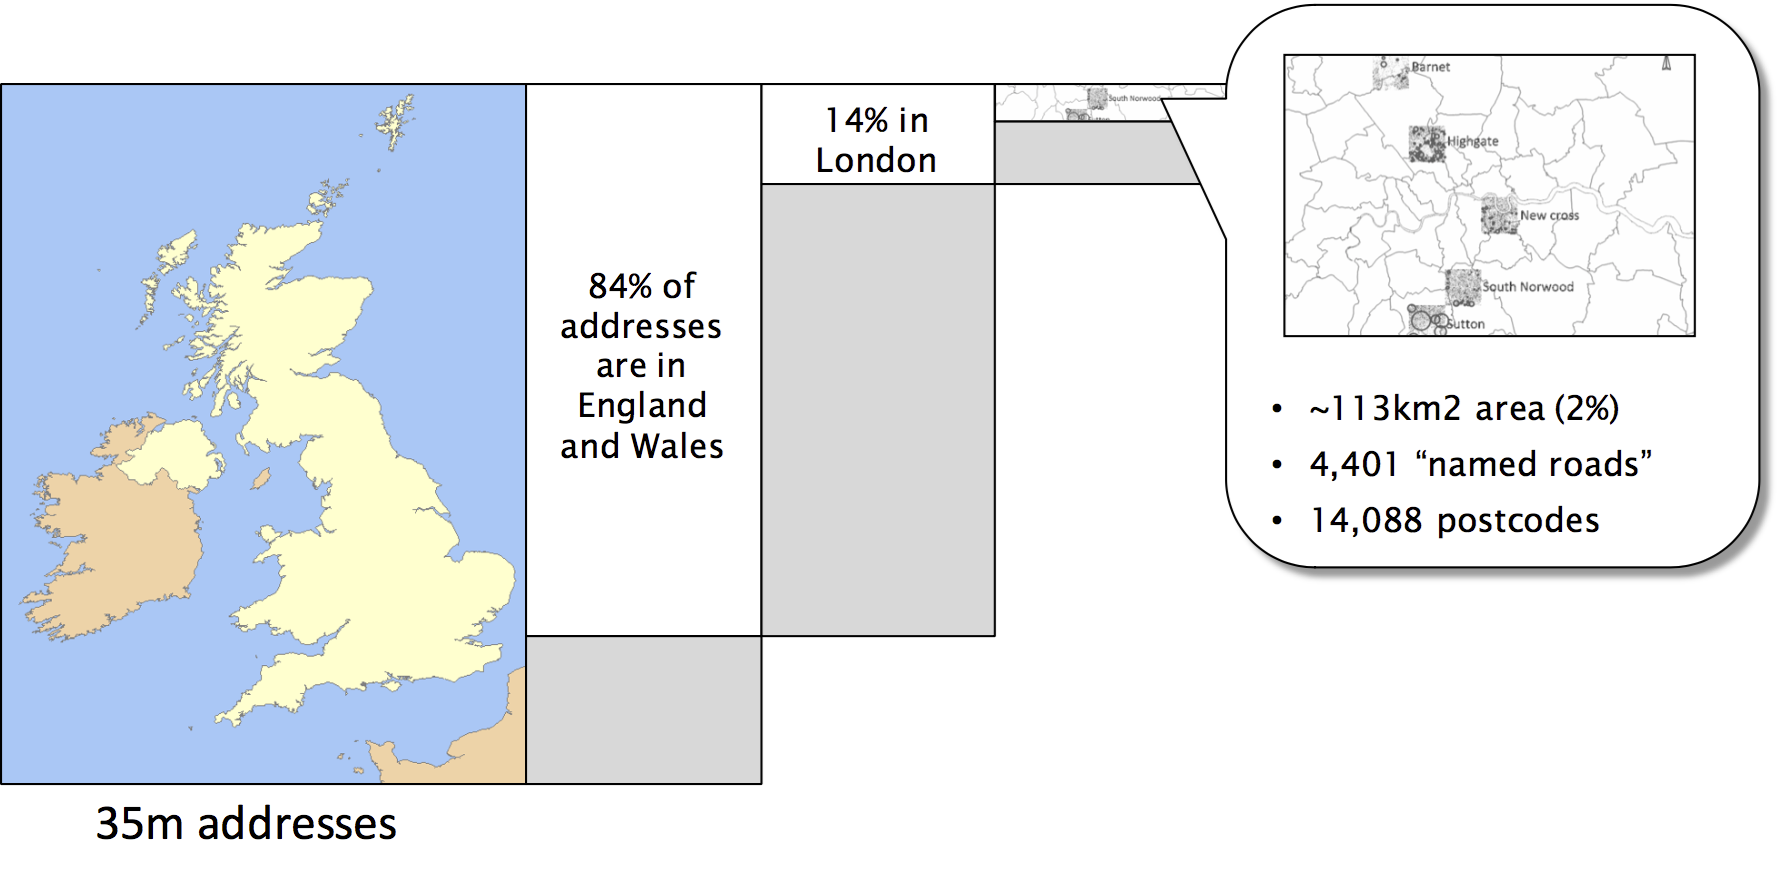
\includegraphics[width=0.50\textwidth]{social-machine-mix-3.png}}{\caption{Applicability of address inference - General statistics}\label{fig:social_machine_mix_3}}
        \ffigbox{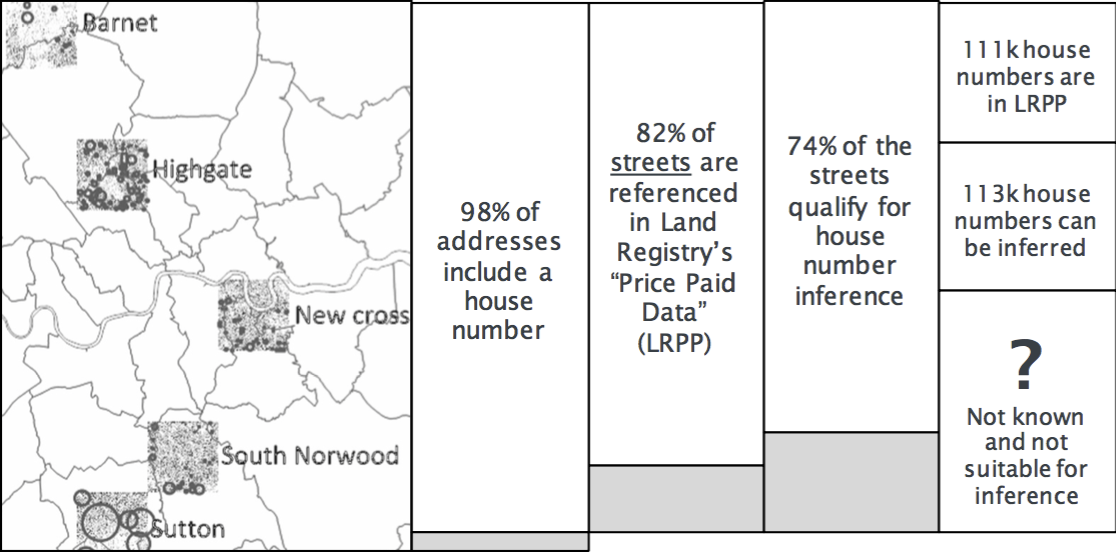
\includegraphics[width=0.40\textwidth]{social-machine-mix-2.png}}{\caption{Applicability of address inference - Sample statistics}\label{fig:social_machine_mix_2}}
   \end{floatrow}
\end{figure}
        
The focus going forward is on the latter problem. Using inference to create the largest sets of inferred house numbers translates into finding out the lowest and highest house numbers the algorithms could be applied to\footnote{For simplicity, we did not consider (a) that it is also useful to know if the streets have both odd and even house numbers and (b) the case where one house number only is known for a street, for which we could assume 1 to be the lowest house number.}.

As no pre-existing open data is available by definition to address this problem, the needed data needs being generated through surveying. 

\subsubsection{{\it p1.4}: Correct the output of {\it p1.2} through surveying.} 

Finally, problem {\it p1.4} is about correcting error in {\it p1.2}, typically identifying house numbers that were inferred but do not exist, or that are replaced by house names.
        
As no pre-existing open data is available by definition to address this problem, the identification of error and the data needed for correction needs being obtained through surveying. 

Problem {\it p1.4} is not discussed in this paper.

\subsection{Crowdsourcing house numbers to enable inference}

The focus of the research described in this paper is the solution of problem {\it p1.3.1}. This is not conceptually different than an annotation problem where for each annotated instance there is a single right answer, with a few key differences:
    
\begin{itemize}
        
    \item For each item subject to annotation, two independent annotations are collected: the lowest and highest visible house numbers. 
        
        There is no use in splitting the task in two, asking one Worker to look for the lowest house number and another to look for the highest. By exploring the pictures of the assigned street the Worker will naturally focus her research on the extremities of the road, where the relevant house numbers are, without knowing in advance which of the two she is finding.
        
        One could argue that the two annotations are not truly independent, as the lowest house number is, by definition, lower than the highest house number. In practical terms, though, the task of surveying a street cannot leverage such mathematical relation. For example, knowing the highest house number won't help the Worker finding the lowest house number, as her finding is rather due toto the observation of the morphology of the street and the progression of nearby house numbers. 
        
    \item The information subject to the annotation could be identified as existing, but the annotation may not be possible anyway. E.g. a Worker will be able to see which the first house in a street is from observing the house numbers on nearby buildings, but vegetation may hide the number. There is also the possibility that Google Street View coverage does not include the surveyed street.
        
        Moreover, unlike other countries, in the UK local authorities do not provide house number plates to the building owners, so this remains their responsibility. Building owners have the option not to affix any plate at all. 
        
    \item There may be nothing to annotate. Because of the nature of the problem, the streets we are using crowdsourcing to collect data about are the ones that appeared little or not at all in pre-existing data, e.g. in Land Registry's Price Paid data over the last 20 years. There likely is a reason for that, e.g. the street may be rural and have few buildings. 
        
\end{itemize}
    
The following is a description of the approach that was used for crowdsourcing addresses, that is common to all experimental conditions that were tested.

\subsubsection{Task model} \leavevmode \\ %% Why is this necessary to get a new line?

\textbf{Requester.} The Requester desires to gather the lowest and the highest house numbers that can be observed in a specified street, as they can be intelligibly identified by browsing pictures of the street. Alternatively, if no two house numbers are identifiable, the Requester needs being informed, too. Different streets have different degree of interest to the Requester, who is interested in prioritising the collection of the data for the higher interest streets in respect to the lower interest ones. The Requester requires the help of human agents to carry out the tasks, that we will call Workers in the following.

\textbf{Task.} Each HIT (Human Intelligence Task) consists of browsing the pictures of a street until achieving reasonable certainty of having identified the lowest and the highest house numbers or, alternatively, the lack thereof.

\textbf{Strategy.} 
The strategy relies on traditional crowdsourcing techniques for image labelling.

\textbf{Crowd $\rightarrow$ Worker.} Each Worker provides judgement on a task by browsing the pictures and declaring if she has found the lowest and the highest house numbers or none. Multiple Workers are asked to identify the house numbers for the same street. The resulting data is chosen through majority voting. We use CrowdFlower as our crowdsourcing platform, presenting each task by embedding customised Google Maps and Google Street View applets into web pages built using the system's templating system. 

\textbf{Quality.} Quality is defined by a combination of (a) accuracy of the Workers in responding to tests questions, and (b) consensus in the data submitted through repeated surveys of the same road. Aggregation takes place accordingly as explained below.

\subsubsection{Workers quality}
    
Probing Workers using conventional test questions - e.g. where the correspondence of the Worker submissions is checked vs the same data collected by the research team as described in \cite{Kittur:2008gj} - would be a powerful tool to identify high vs low quality Workers, but is very expensive in OLAF's case. The task of surveying a street is not trivial, and early anecdotal evidence showed many Workers leaving after performing no more than two or three surveys. To further damage the performance of the system, the ones who stayed longer started cheating, or showed a substantial drop in their performance. This suggested that spending a substantial part of the Worker's effort on test questions - e.g. making one out of three surveys a test - was not affordable.

Not using any kind of test question is unlikely to be successful, too, and it was explored in previous work such as \cite{DellaPenna:tf} [THIS PAPER ACTUALLY THEORISES THE IMPOSSIBILITY OF GOOD RESULTS WHEN WORKERS HAVE ACCESS TO COMMONLY SHARED PREJUDICE: COULD THIS BE EQUIVALENT TO THE CASE WHERE MY WORKERS ALL END UP BELIEVING THAT SOME EASILY ACCESSIBLE AND VISIBLE CORNER OF A STREET HAS THE HIGHEST HOUSE NUMBER, BUT THE REAL ONE IS ELSEWHERE?]. As an alternative, though, simple test questions can be set up on data that is already available, in a way that is similar to classic anti-spamming techniques like CAPTCHAs as described in \cite{Difallah:2012ty}. In OLAF's case the name of the street itself is used: Workers are asked to copy and paste or type the name of the street as part of their survey. Workers that do not achieve the target accuracy are excluded from further work.

\subsubsection{Results aggregation}

Repeated surveys are equivalent to the use of repeated judgement in conventional image labelling exercises. These have been explored extensively in literature and demonstrate that the results produced by a few expensive expert individuals are comparable to what emerges from involving multiple answers by crowds of non-expert Workers, e.g. in \cite{Snow:2008wo} and \cite{Sheng:2008gra}. As the answers are inevitably noisy, different Workers were asked to survey the same road, and their responses are aggregated to decide what is the most likely and truthful observation. 
        
Approaches to aggregation are an equally well studied subject, and a majority decision is a natural option (e.g. \cite{Le:2010ug}). The detailed parameters and process of how consensus is defined and calculated are tuned for better performance and address issues specific to the context (e.g. in \cite{Hirth:2011fh}). 

In the case of OLAF, consensus is measured by using Fleiss' kappa statistics for inter-annotator agreement, as described for example in \cite{Nowak:2010gt}. For those streets where the house numbers {\it were} stated to be found, a kappa of 60\% on at least 5 surveys is sufficient consensus (e.g. see \cite{Landis:1977kv}). For those streets where the house numbers were stated {\it not} to be found, a kappa of 80\% on at least 10 surveys is required instead, as it is more likely that unreliable Workers agree in reporting that.

The number of 5 and 10 judgements is chosen because they are respectively the minimum number of judgements where 60\% and 80\% kappa can be achieved without the need of an unanimous agreement (4 vs 1 for 60\% and 9 vs 1 for 80\%). 

Rounds of 5 surveys per road are performed until consensus is reached on both its lowest and highest house numbers. Because of the nature of the task, new surveys are performed even if consensus is reached already on either of the two numbers.  

\subsubsection{Recruitment}

We sourced all our Workers from CrowdFlower. For each experiment, we created one dedicated CrowdFlower job. We used identical settings for each experiment set, consisting of the following parameters:

\textbf{Geography} Limited to the top 10 contributor countries in CrowdFlower where English is an official or officially recognised language\footnote{See \url{https://success.crowdflower.com/hc/en-us/articles/202703345-Crowd-Demographics}, the identification of the countries was last repeated on 19 December 2015, before the running the experiments described in this paper. The list of countries is: Bangladesh, Canada, India, Malaysia, Netherlands, Pakistan, Philippines, Sri Lanka, United Kingdom and United States of America.}.

\textbf{Skills} We chose Workers from the default CrowdFlower performance category (formerly named "level 2"), that accounts for 29\% of the total population\footnote{See \url{https://success.crowdflower.com/hc/en-us/articles/202703345-Crowd-Demographics}, the calculation was done on 19 December 2015.}[MORE INTERESTING TO KNOW THE VOLUME OF JUDGEMENTS THEY MAKE, THE OLDER CROWDFLOWER UI SEYI USED GAVE THIS INFORMATION].

\textbf{Accuracy} As described in the previous section, as a test question Workers were asked to copy and paste or type the name of the street as part of their submission in each task. Being the question this simple, error was not accepted the requested accuracy was 99\%\footnote{CrowdFlower does not allow the Requester to set target accuracy to 100\%.}.

\textbf{Judgements} In groups of 3 per road, repeated until consensus is reached, by different Workers without repetition. Each worker is allowed to contribute to a maximum of 10\% of the streets available to survey at each round.

\textbf{Behaviour} Each Worker was paid for 1 task, and 1 task is made of 1 street to survey.

\textbf{Reward / Time Limits} The reward was 0.34 US Dollars per task. Workers requiring less than 90 seconds per task were considered at high risk of being malicious and excluded to perform additional tasks. CrowdFlower imposes a time limit of 30 minutes maximum per task[NEED TO CHECK THIS].

\subsubsection{Design}
\subsubsection{The data processing solution}

All of the data required to setup the crowdsourcing operation is created from the original distributions by Ordinance Survey and Land Registry. 

The data is stored in a PostgreSQL database\footnote{See \url{http://www.postgresql.org/}.}, that was chosen mostly for its robust and well documented PostGIS extension\footnote{See \url{http://postgis.net/}.}, providing geospatial data processing functionality. NodeJS\footnote{See \url{https://nodejs.org}.} and PostgreSQL scripts were used to import and process the data end to end, up to the point where it is exported to the virtual survey tool, described below. Although the volume of the data being processed is not small, it's far from requiring the tools typical of big data applications. 

The full code is available on GitHub in three repositories:

\begin{itemize}
    \item To import and filter the source Ordnance Survey and Land Registry data in what is then used by the experiments as reference: \url{https://github.com/Digital-Contraptions-Imaginarium/OLAF-yr2_reference_data}
    \item To calculate address inference from the above: \url{https://github.com/Digital-Contraptions-Imaginarium/OLAF-yr2_inference_data}
    \item To consolidate and prepare the data for uploading into the virtual survey tool: \url{https://github.com/Digital-Contraptions-Imaginarium/OLAF-yr2_lab/}.
\end{itemize}

\subsubsection{The virtual survey tool}

The virtual survey tool is built exclusively by using the native functionality of two highly available and scalable cloud systems: CrowdFlower and Google Maps and Street View APIs. 

CrowdFlower\footnote{See \url{http://www.crowdflower.com/}.} is a common choice among crowdsourcing services outside of the US\footnote{Differently than Amazon Mechanical Turk, CrowdFlower users are not required to provide an US-registered payment card for registration.}. It offers a full end-to-end solution to run crowdsourcing campaigns, including the recruitment, profiling and management of the Workers, a few tools for quality control, the payment system and the hosting of the actual website through which the Workers contribute. Optionally, some or all of its services can be integrated through APIs into systems owned by its clients. CrowdFlower's particularly suitable to the delivery of open data initiatives as its services are available for free - but for the Workers' compensaton - by choosing their "Data for Everyone" plan, where CrowdFlower reserves the right to publish the data collected through the crowdsourcing jobs. To keep the overall system as simple as possible - while highly scalable and available - it was decided to rely on CrowdFlower's native functionality only and design the system within the limitations of its customisation features.

The Google Maps and Street View APIs\footnote{See \url{https://developers.google.com/maps/web/}.} allow to embed fully featured interactive maps as part of third party websites. They provide out of the box powerful customisation features through JavaScript scripting, some of which were implemented for the survey tool, such as limiting the user freedom of movement within the maps to the bounding box that contains the street subject to surveying.   

Below is how the tool looks like to a first time user.

\begin{figure*}
	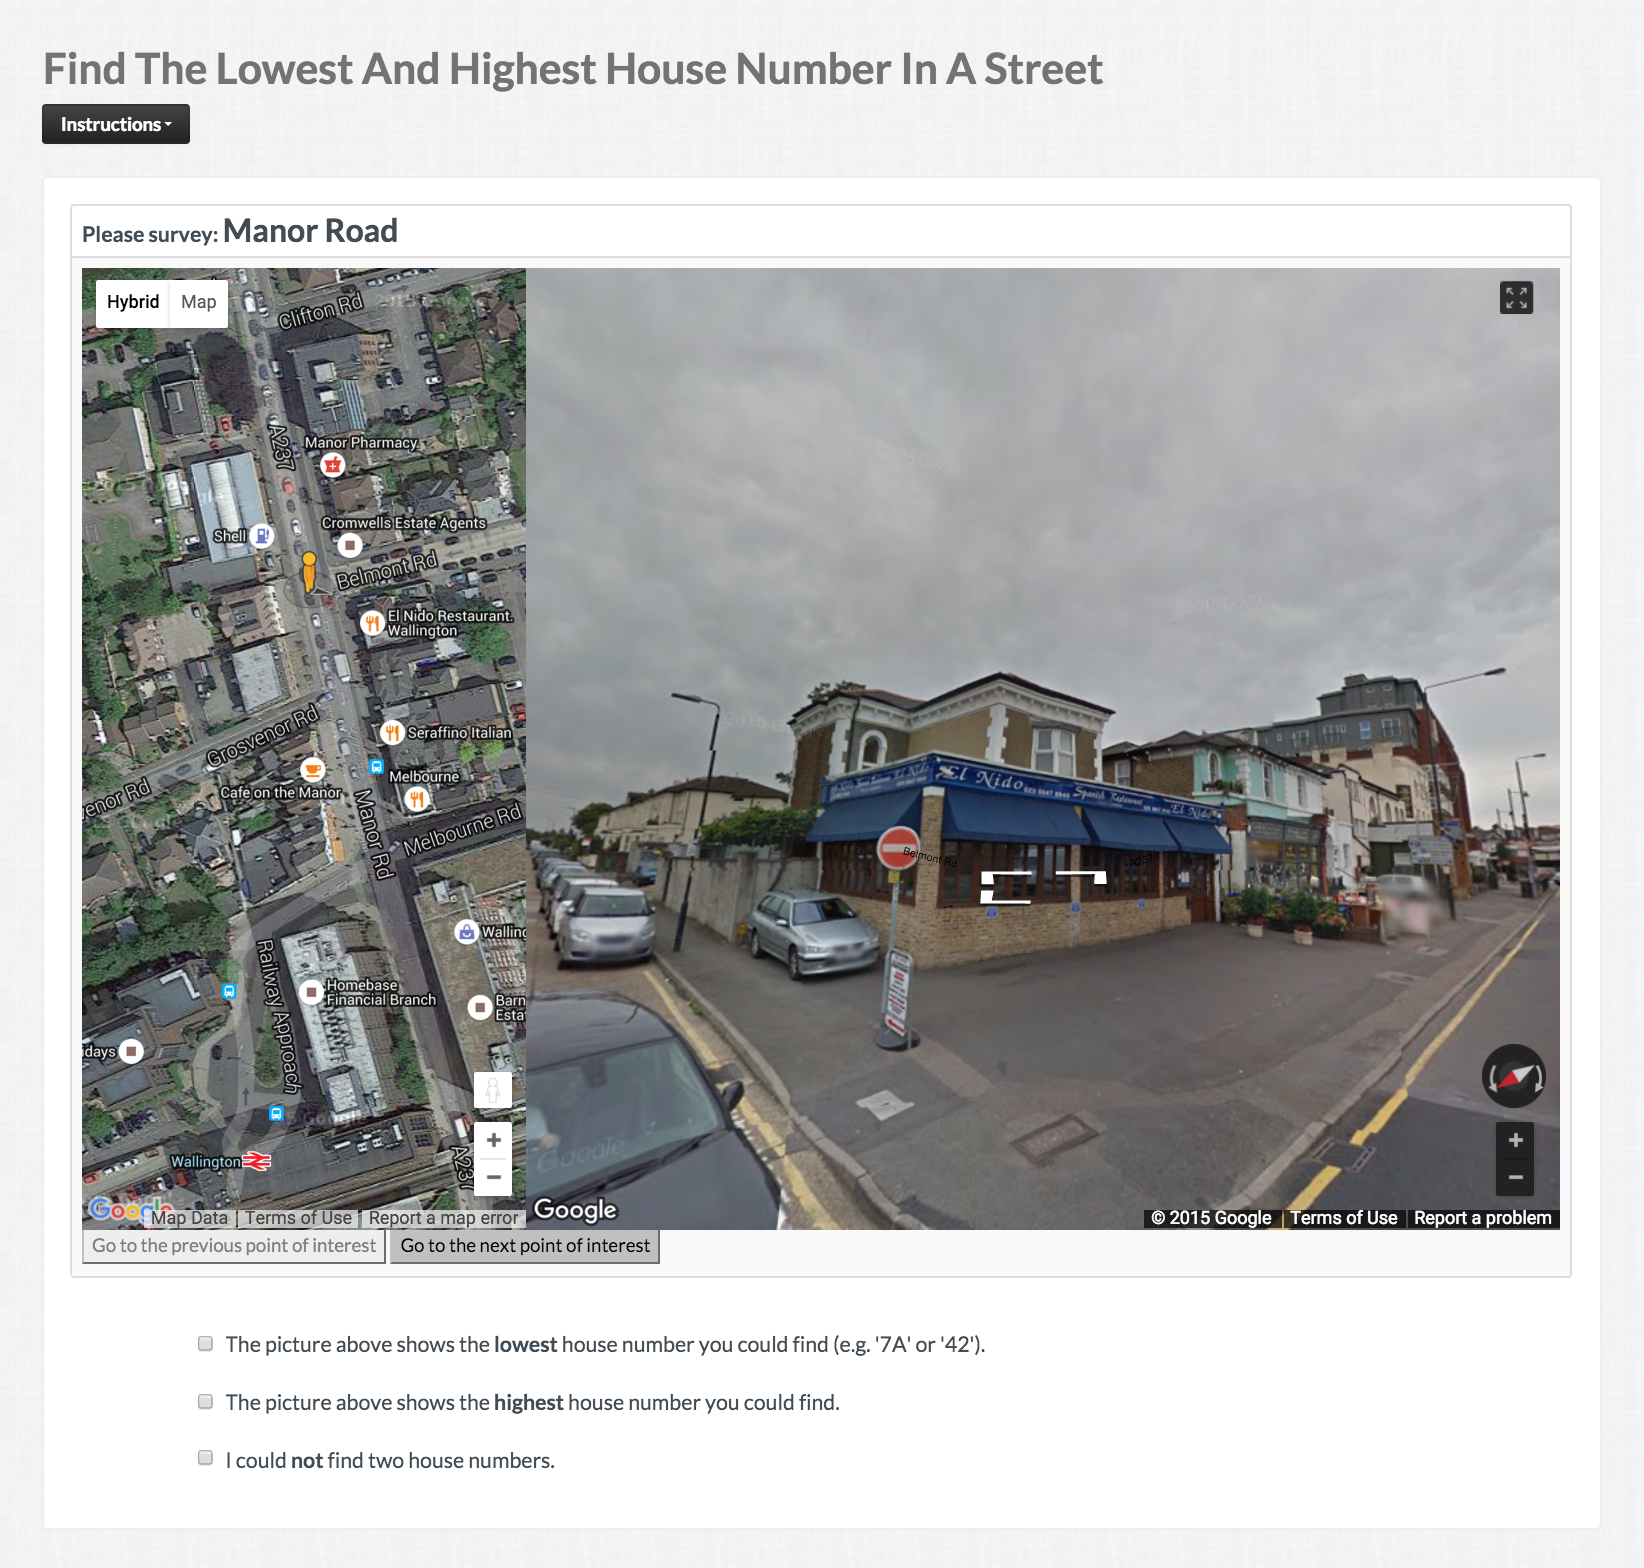
\includegraphics[width=0.95\textwidth]{virtual-survey-tool-01.png}
	\caption{This picture should not be here, but apparently it is a nightmare in LaTeX.}
	\label{fig:some_figure}
\end{figure*}

\paragraph{}

The full code is available on GitHub at \url{https://github.com/Digital-Contraptions-Imaginarium/OLAF-yr2_lab/}.

\subsection{Implementation}


(i) ingestion and preparation of the reference data\footnote{See the GitHub repository at \url{https://github.com/Digital-Contraptions-Imaginarium/OLAF-yr2_reference_data}.}, (ii) inference of house numbers where made possible from LRPP data\footnote{See the GitHub repository at \url{https://github.com/Digital-Contraptions-Imaginarium/OLAF-yr2_inference_data}.} and (iii) creation of the data for the crowdsourcing component and elaborating its results\footnote{See the GitHub repository at \url{https://github.com/Digital-Contraptions-Imaginarium/OLAF-yr2_lab}, {\it data-prep-scripts} and {\it analysis-scripts} folders respectively.}. 


    	
    \subsubsection{Scalability}
    
        [THE CALL FOR PAPER EXPLICITLY SAYS THAT "EVIDENCE OF USE IN PRACTICE AND/OR DEMONSTRATION OF SCALABILITY IS REGARDED AS A PLUS"]
    
    \subsubsection{{[}description of additional conditions to test X{]}}
    \subsubsection{{[}description of additional conditions to test Y{]}}

[FIND SOME PLACE TO SAY WHY WE DON'T USE OPENSTREETMAP, BECAUSE SOMEONE WILL ASK. THE ANSWER IS THAT ITS LICENSING IS CONTROVERSIAL ACCORDING TO SOME: E.G. READ \cite{CentreforSpatialLawandPolicy:2014tx}]
    

